\chapter{Course Staff's Guide to Diderot}
\label{ch:guide}

\begin{preamble}
This chapter describes common course management workflows for instructors and teaching assistants.
\end{preamble}


\section{Course Home Page}

\begin{gram}[The Zones]
Course home page, shown below, consists of four zones.
\begin{enumerate}
\item A toolbar, at the top
\item A ``news'' or ``Latest Announcements'' area on the top left quadrant.
\item Quick links on the right top right quadrant.
\item The books, an the lower half.
\end{enumerate}

You can go to the course home page by pressing the ``Home'' button at the top right corner.

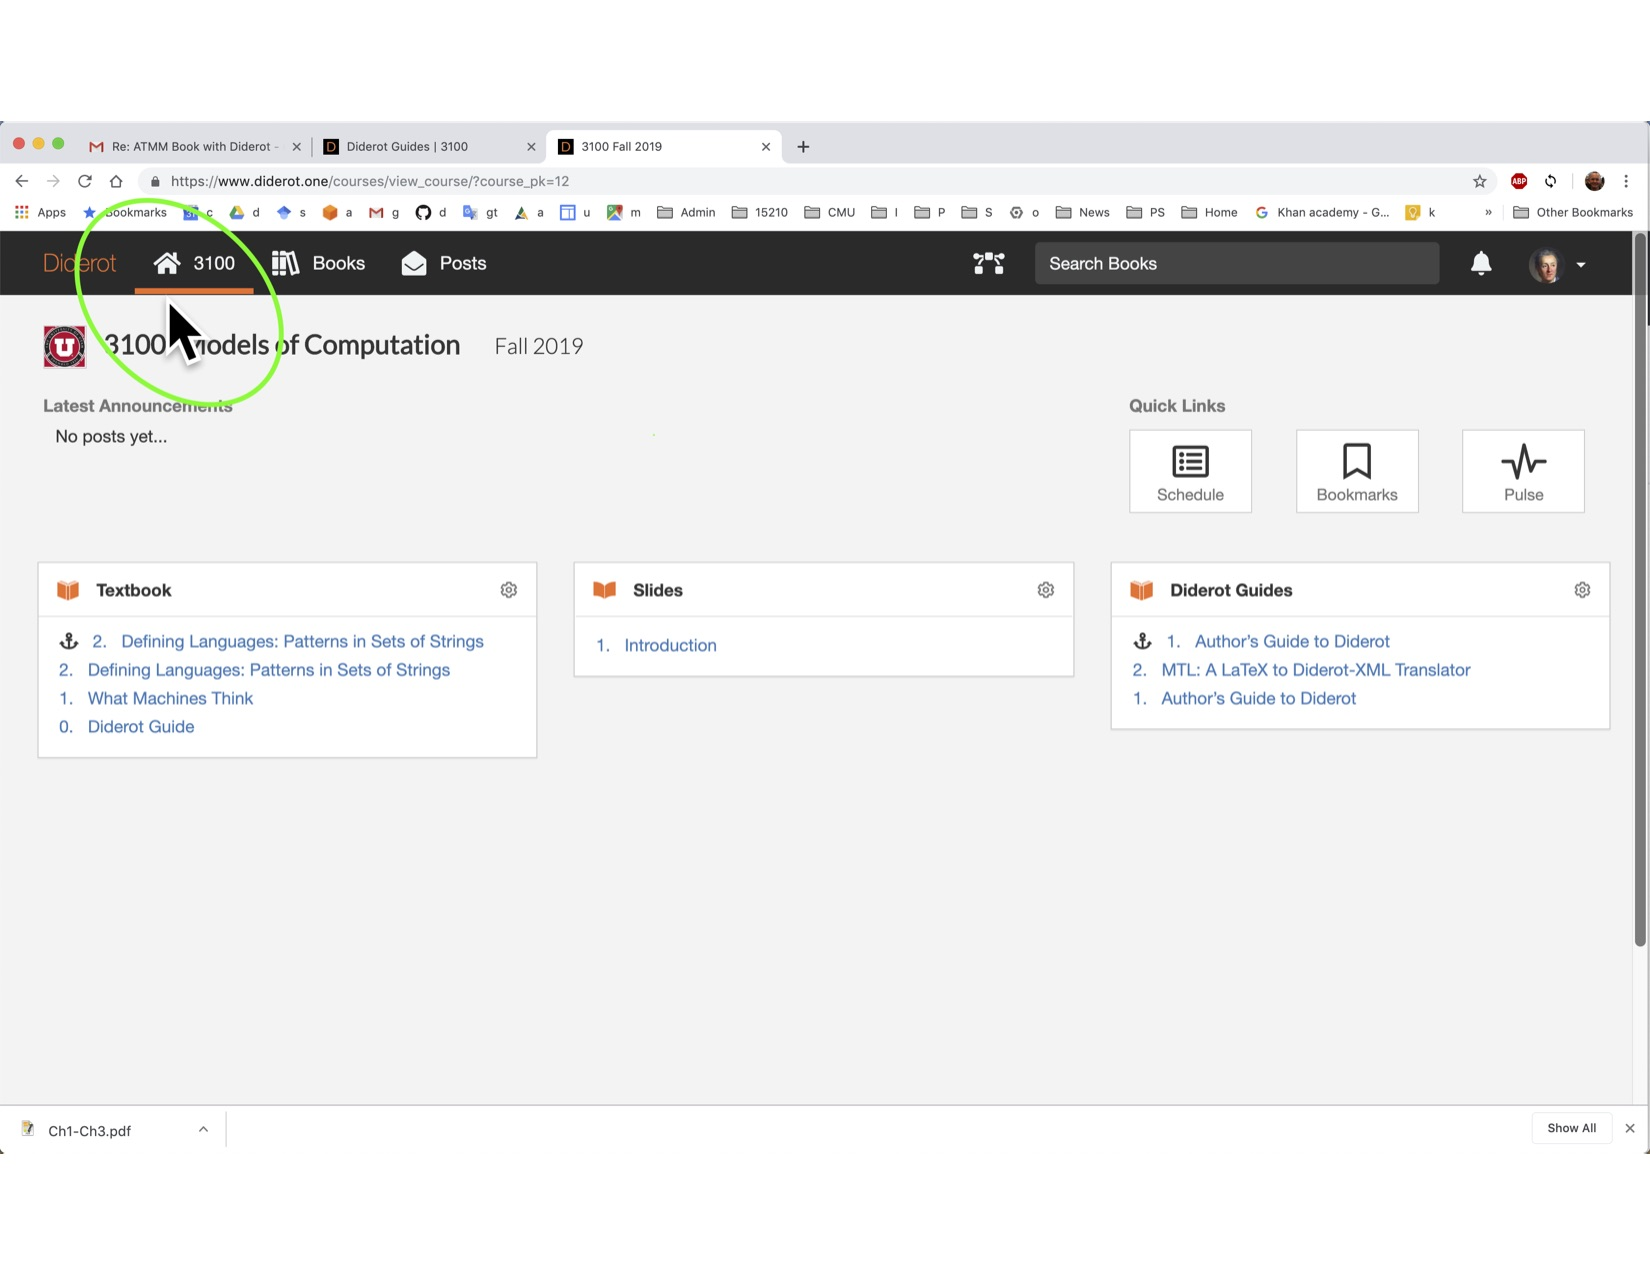
\includegraphics[width=0.9\textwidth]{staff/media/course-home.jpg}
\end{gram}

\section{Book Management}

\begin{gram}[Finding Book Management]
\label{guide::author::go-book-management}
As an author, you will spend much of your time in the ``Book Management'' page.
A quick way to get to this page is to go to the course home page and to press the settings (``wheel'') icon for the book that you want to manage.
%
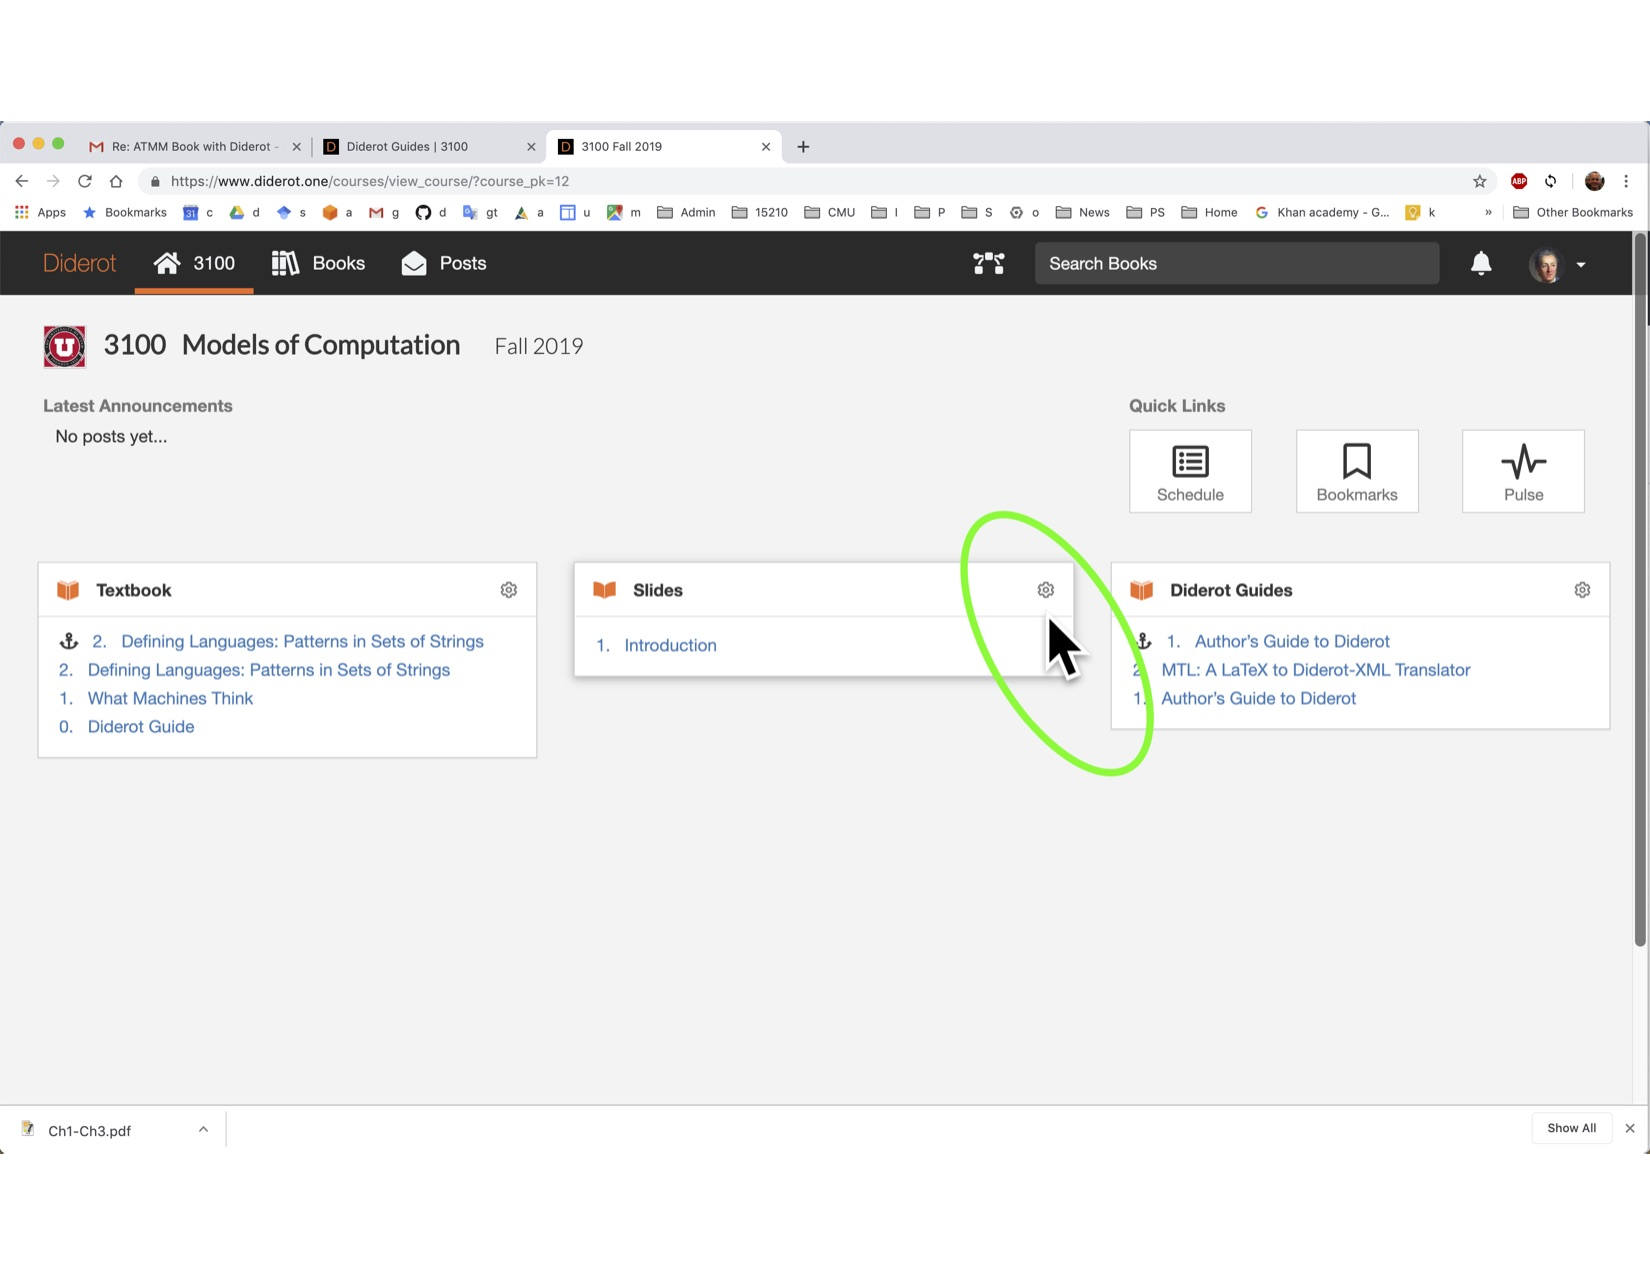
\includegraphics[width=0.9\textwidth]{staff/media/go-to-book-management.jpg}
\end{gram}


\begin{gram}
The book management page offers functionality for
\begin{itemize}
\item creating chapters,
\item uploading content onto chapters,
\item realeasing/unreleasing chapters,
\item deleting chapters,
\item additional more advanced operations, which we will skip for now.
\end{itemize}

To see the actions that you can perform on a chapter options, move the mouse over to that chapter. 

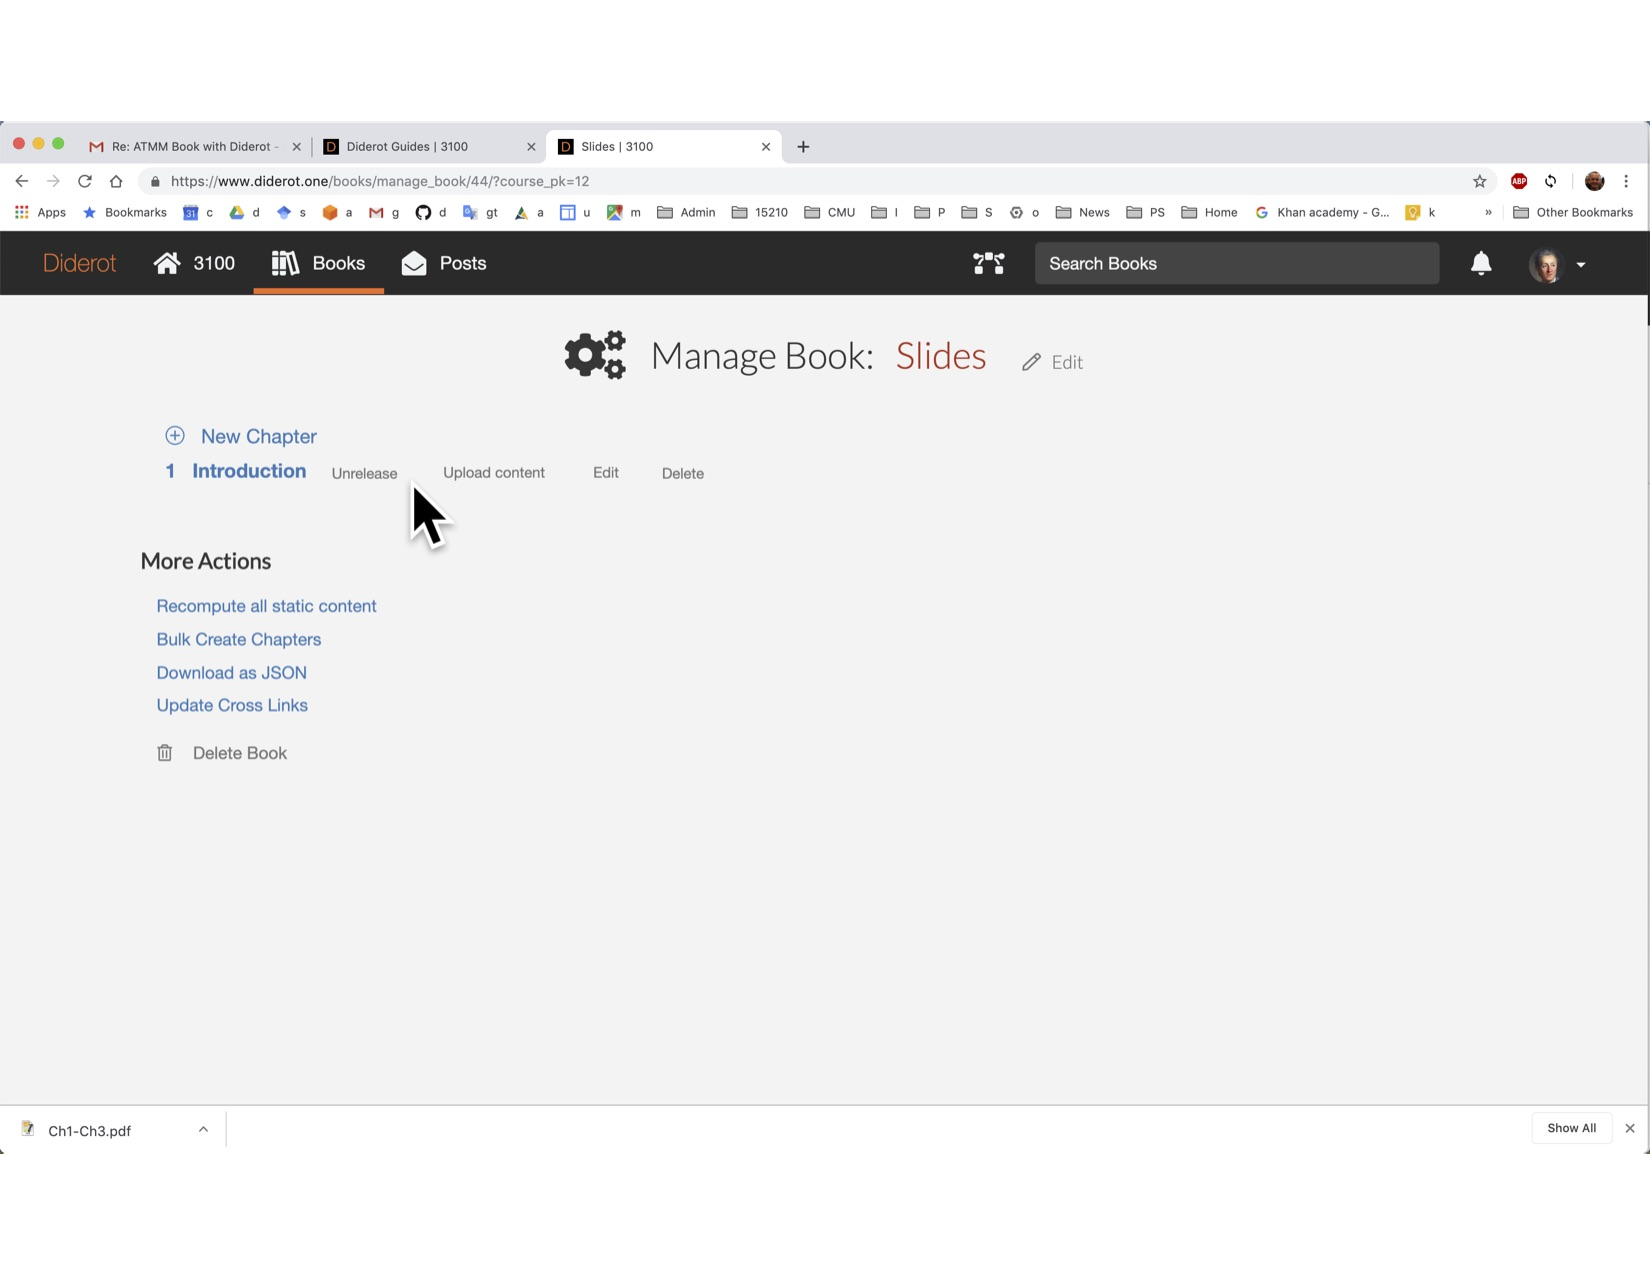
\includegraphics[width=0.9\textwidth]{staff/media/book-management.jpg}
\end{gram}

\begin{exercise}
Create a book called ``Slides'' for uploading some slide decks. 
\begin{enumerate}
\item Go to "Manage Books" from the "Links" on the center right, to
the left of search bar on top.
\item Create the book ``Slides''.
\end{enumerate}
\end{exercise}

\section{Chapters}
\label{guide:chapter}

\begin{gram}[Chapter Creation]
\label{guide:chapter::create}
You can add a chapter to a book.  
\begin{itemize}
\item Go to course home page.
\item \href{guide::author::go-book-management}{Find the book} that you
  want to edit.  You can reach the book management screen from the
  "Manage Books" link from the "Links" button on the center right, to
  the left of search bar on top.

\item  Press ``Create chapter'' and follow the instructions.  To create a chapter in its most basic form, you can leave all of the rest of the fields empty.  The additional field are discussed below.
\end{itemize}
%

When creating a chapter, assign the chapter a unique number and a unique label, e.g., \ttt{ch:kleene}.  
%
The label needs to be unique only within the book---no two chapters of
the same book can have the same label.
%
If the chosen label does not meet this criteria, you will receive an error message and can choose another one.

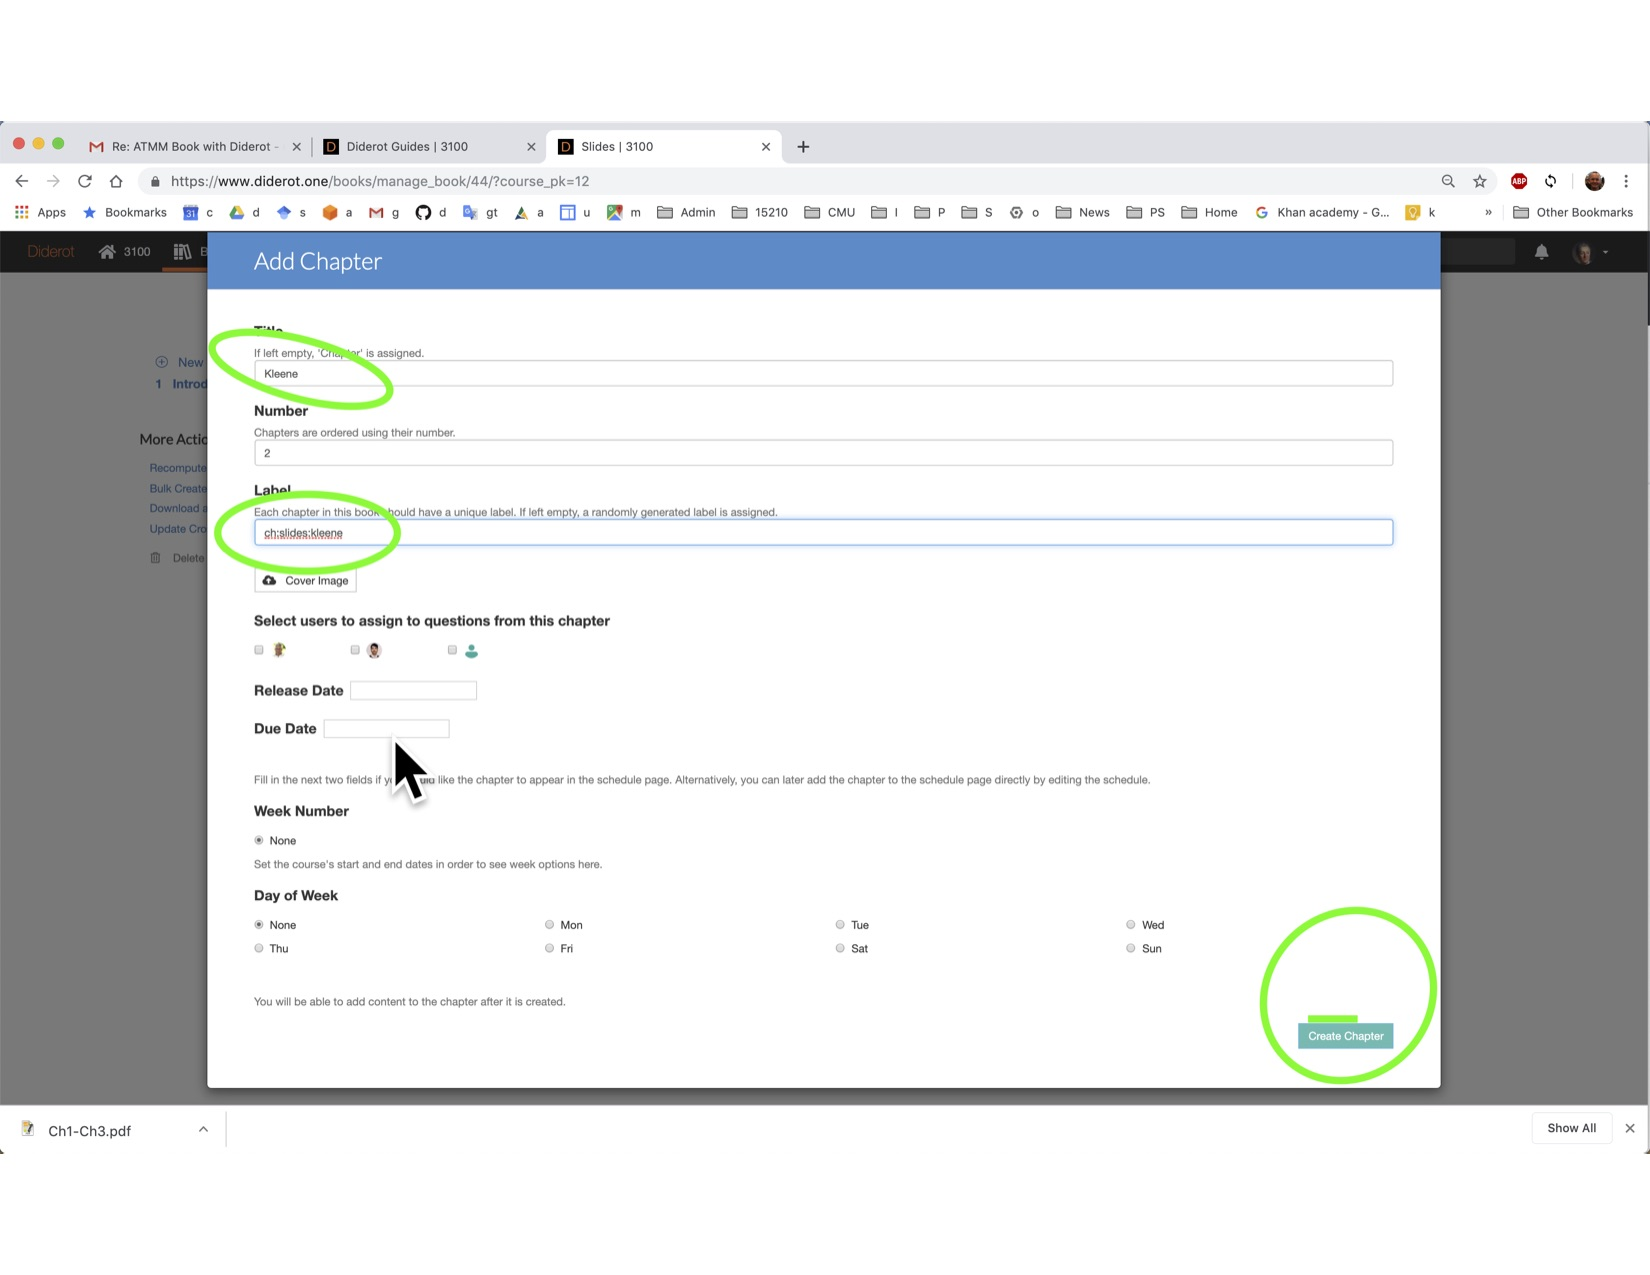
\includegraphics[width=0.9\textwidth]{staff/media/create-chapter.jpg}
\end{gram}

\begin{exercise}
Create a chapter for a slide deck and give it the label
\ttt{ch:test-slides}.
\end{exercise}


\begin{gram}[Released versus Unreleased Chapters]
A chapter is either released or unreleased. 
%
\defn{Released} chapters are visible to the students.
%
\defn{Unreleased} chapters are not visible to the students but  are visible to course staff.  

This is designed to allow for a ``feedback cycle'' before releasing chapters to students.  
%
For example, I typically  upload my lectures a bit ahead of time and before releasing them, ask my TAs to look over them and give feedback.
%
To give feedback, the TA's simply select the relevant atom and create a feedback, e.g., they might note a typo.
%
I then fix these problems, reupload the chapter, and then release it.  
\end{gram}

\begin{gram}[Release Dates and Schedule]  
You can assign release dates to your chapters and this will
automatically construct (and maintain) a schedule for you.  Let's skip
this step for now.  So leave these fields empty.  You can edit
chapters to add schedule information later.
\end{gram}


\begin{gram}[User Assignments]
You can "assign" users to a chapter.  The intention here is to
designate \defn{discussion chairs}, who are usually TAs for each
chapter. 
%
They will be assigned the questions asked on that content.

I don't know who I will assign the chapters to at the time of creation and therefore leave this blank.  I or the TAs later edit the chapter to assign the discussion chairs. 
\end{gram}

\begin{gram}[Upload Window]
\label{guide:chapter::upload::window}
To upload contents into a chapter, move the mouse over the chapter and
select upload content.  Here you can upload either an XML
file or a PDF.  
\end{gram}

\begin{gram}[PDF Uploads]
\label{guide:chapter::upload-pdf}
To upload a PDF document bring up the upload window and  select 

\begin{itemize}
\item ``Upload PDF Slides'', or 
\item ``Upload Regular PDF.''
\end{itemize}

Then select the PDF file to upload, and press ``Upload Content''.

Now you will see a spinning wheel.  This will take some time maybe a
minute or two.  What is going on is that the PDF is split into pages
and the text is extracted from it.  When it is finished, click on the
chapter and you should be able to view it.  

As an example, upload your second slide deck from your Fall 2018 site to the chapter that you have created above.

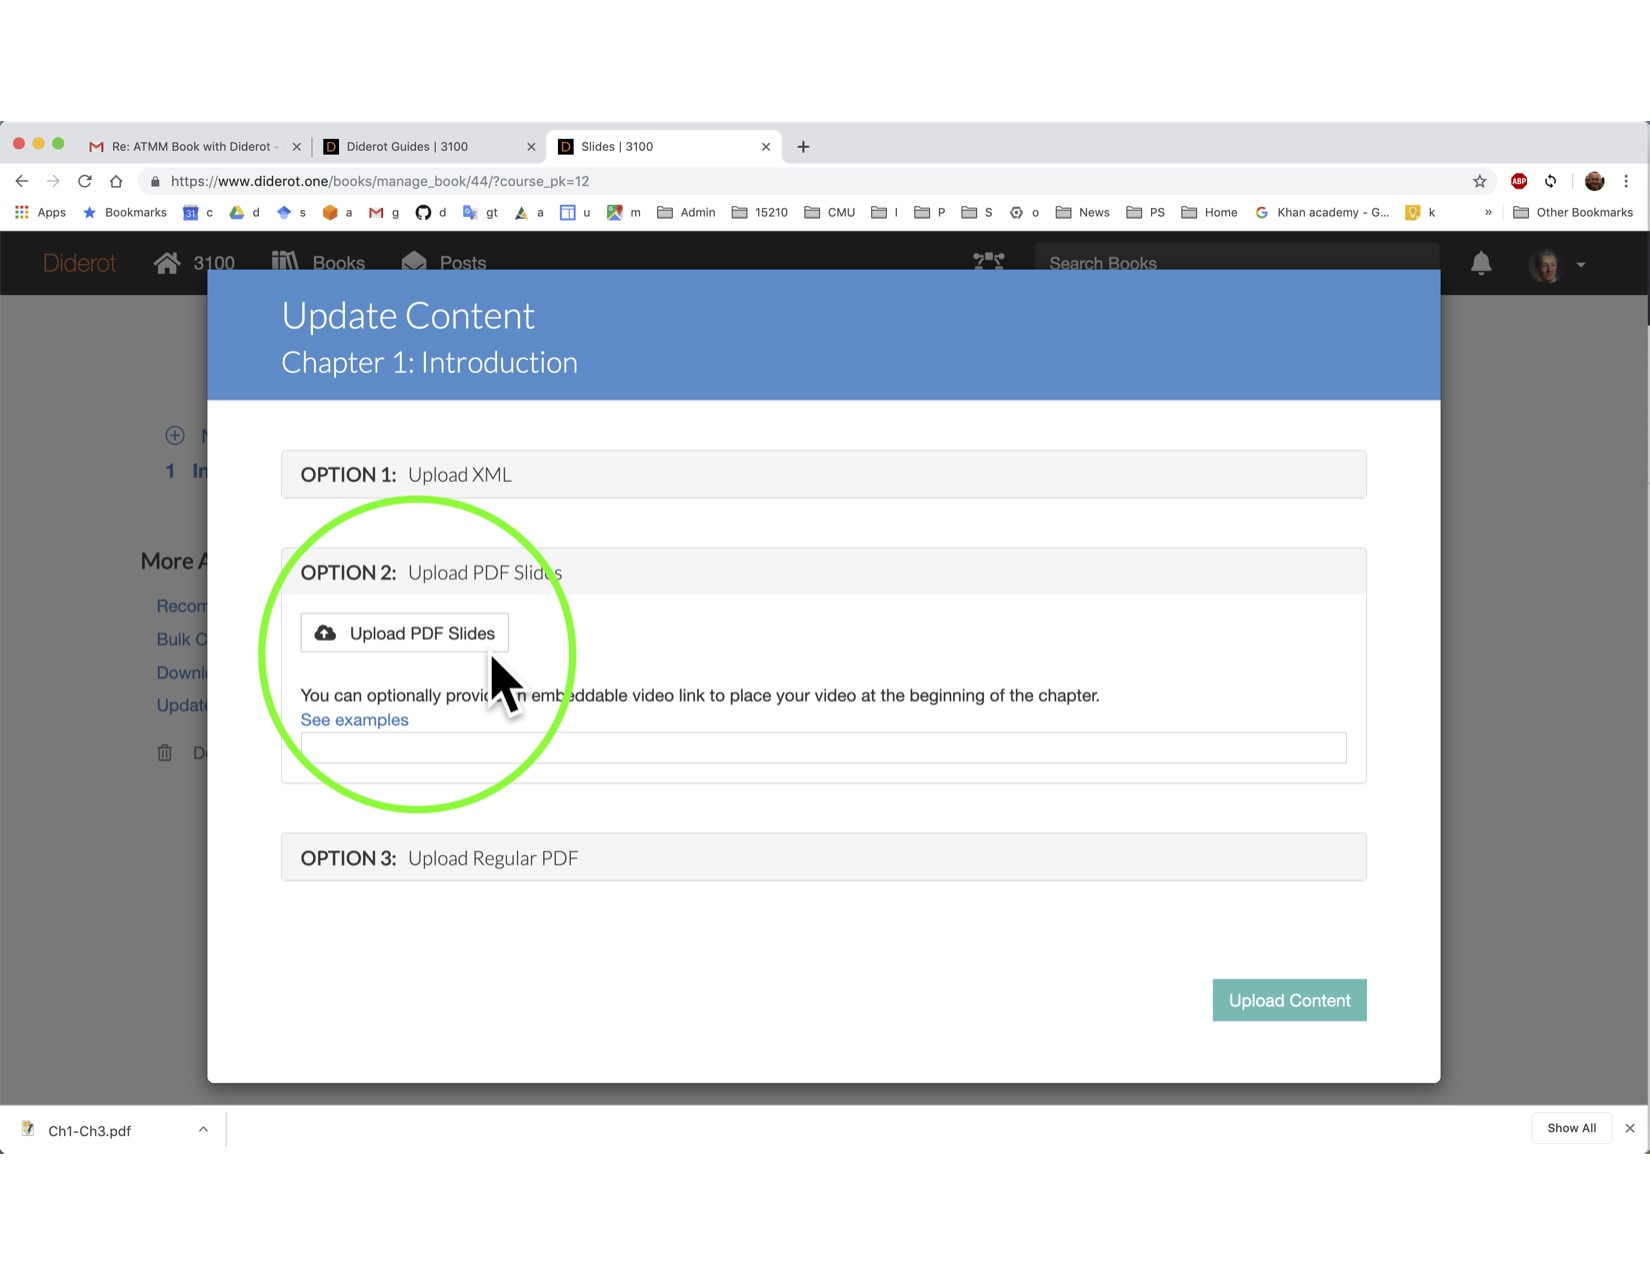
\includegraphics[width=0.9\textwidth]{staff/media/upload-slides.jpg}
\end{gram}


\begin{gram}[XML Uploads]
\label{guide:chapter::upload-xml}
To upload a Diderot XML, first use the DC compiler to generate one.  You can generate Diderot XML from LaTeX or from Markdown.  Next, press the ``Upload XML'' and select the XML file that you want to upload. 
%

If your chapter includes images, you can upload the images along with your XML by pressing ``Upload Images'' and then selecting all of the images (multiple images can be selected) that you want to upload.

Now press ``Upload Content''. You will see a spinning wheel.  This will take some time maybe a minute or two.  What is going on is that your XML document is parsed into a tree of a chapter, sections, and atoms and everything is linked so that the images and document links now point to their right places.

When the spin stops, click on the chapter and you should be able to
view it.

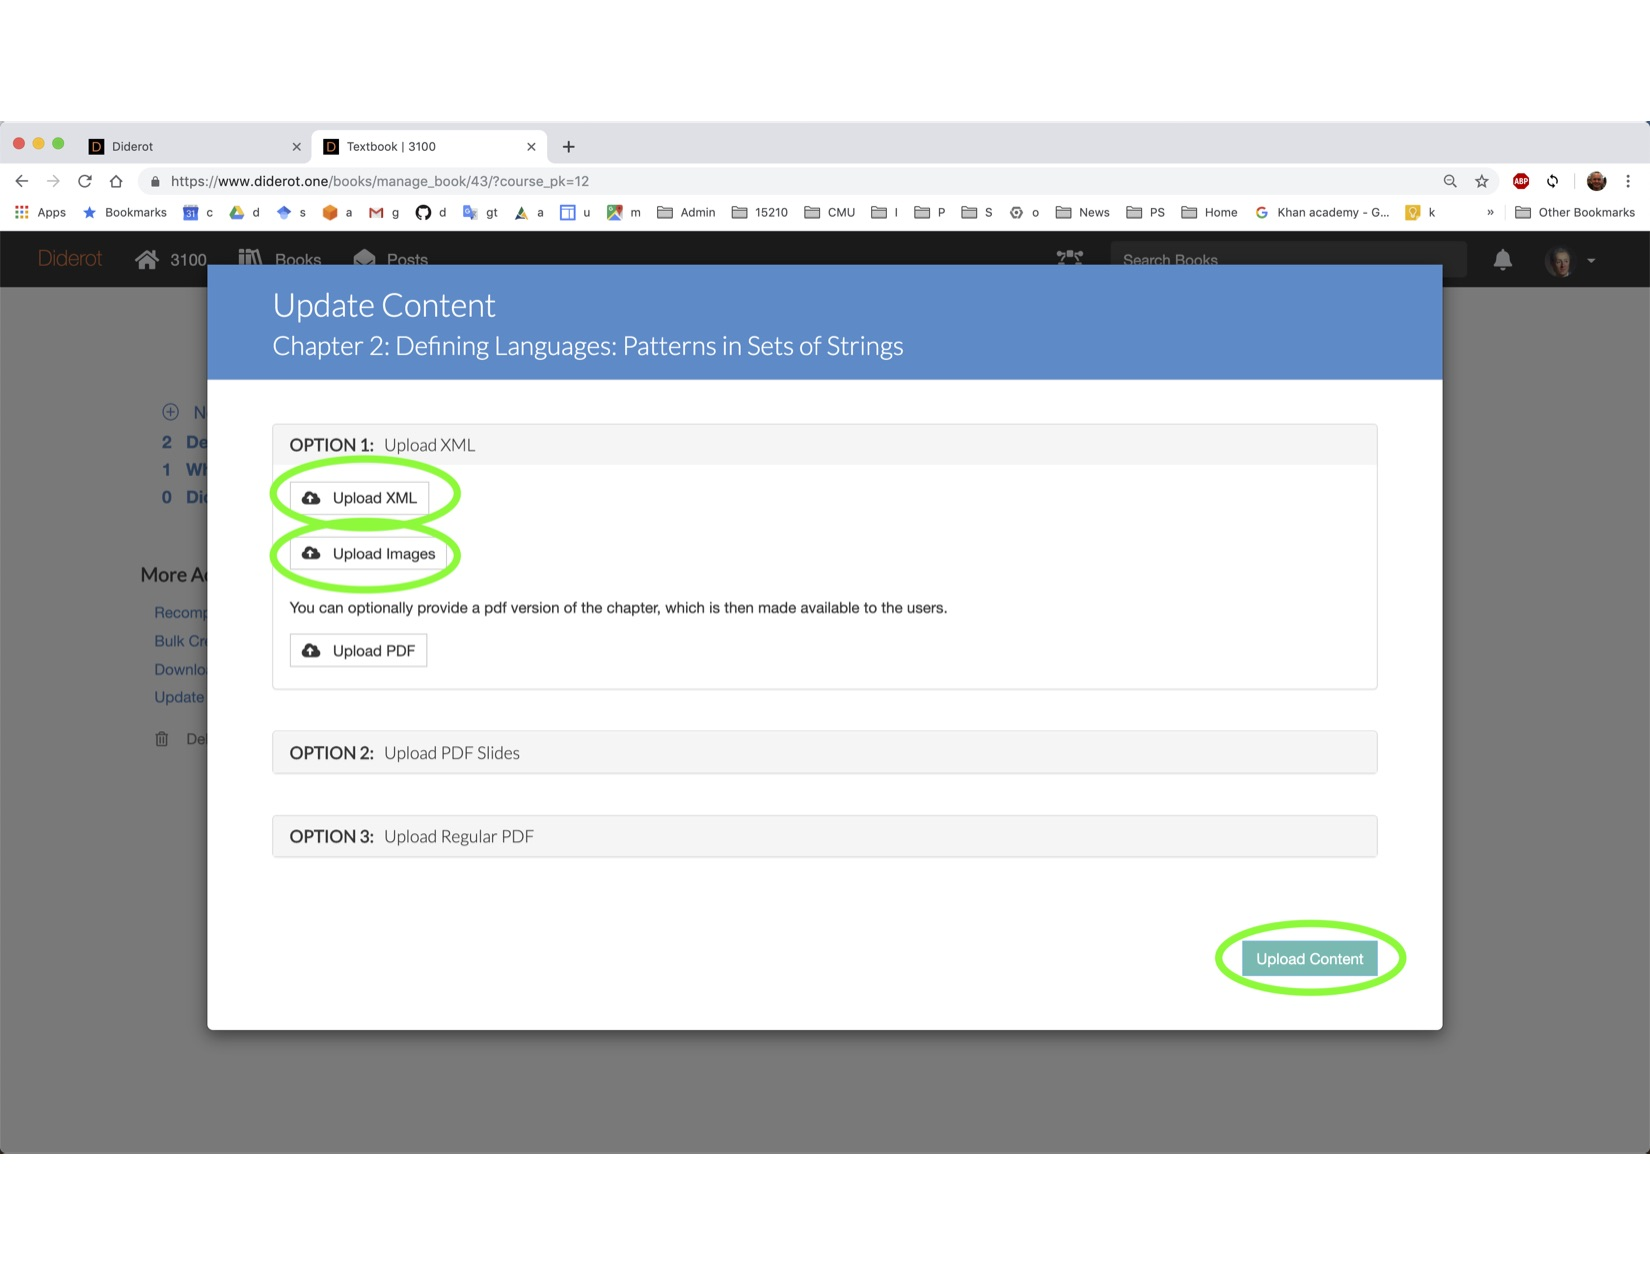
\includegraphics[width=0.9\textwidth]{staff/media/upload-xml.jpg}
\end{gram}



\begin{important}[Unreleased chapters are not searchable]
When a PDF/XML document is uploaded, its contents is stored into an index, allowing it to be searched via the search bar when the chapter is released.
%
Unreleased chapters will not be searchable (so students won't see
unreleased content).
\end{important}

\begin{note}
Currently, pdf documents themselves are shown as JPEG images.  We are in the process of changing this so that they are shows an PDFs.  This should be ready soon.
\end{note}


\begin{gram}[Interactive Chapters]
Once a chapter is uploaded, it becomes interactive.

\begin{itemize}
\item
If unreleased, course staff may send feedback and open other discussions. 
\item
If released: all the students and staff may send feedback, ask questions, take private notes on the content, etc.
\end{itemize}
\end{gram}


\begin{gram}[Updating a Chapter]
For unreleased chapters, simply re-upload the contents.  This will
recreate the chapter and delete all prior discussions on it.  

For released chapters, you can unrelease and re-upload, but this will
delete all content, including student created content (private notes,
questions, etc). 
%
Unreleasing and re-uploading could be thought as the same as deleting the chapter and recreating it.
%
Because it deletes all related content, we discourage using this
feature (after a course starts).  If you don't currently have students and are developing content, you may release chapters, and re-upload them as you wish.

There is only one reliable way to update released content without deletion or without unreleasing it: assign to the chapter, all sections, and all groups, and atoms a label.  This allows Diderot to match the content being uploaded to existing content without ambiguities.  Otherwise, there can be possible ambiguities, because, for example, Diderot doesn't know which updated section corresponds to which existing section. 
\end{gram}

\section{Books}
\label{guide:books}

\begin{gram}[Create a book]
You can create new books and as many as you want.  I usually create one for textbook, one for recitations, one for assignments, one for additional materials (misc).  Many courses create a "Slides" book.  

To create a book go to "links" to the right of the search bar and then press
manage books.  You will give your book a unique label (e.g,
"textbook", "recitations", "misc"...) and a unique"rank" which is the
order it will be shown but is otherwise immaterial.  

By default, a book is selected to be a \defn{booklet}, which
consists of a sequence of chapter.  
%
If you want the book to contain "parts" as an organization element
above chapters, uncheck the ``booklet'' box.  

A book can contain PDFs or XMLs (generated by a compiler).
\end{gram}

\begin{example}
In the algorithms (15210) course, the main textbook has parts but
the rest of the books don't.  So all the books except for the textbook are booklets.
\end{example}


\begin{gram}[Editing a Book]
To edit the book, create and upload chapters, go to "Manage Books" and select your book.  Here you can edit various properties of the book, 
%
\href{guide:chapter::create}{create chapters}
%
\href{guide:chapter::upload-pdf}{upload PDF content}, and
\href{guide:chapter::upload-xml}{upload XML content}.
\end{gram}


\section{User Accounts} 

\begin{gram}[Creation]
To create user accounts, you can upload a roster in CSV format, which will email them all.
%
\begin{enumerate}
\item
Go to ``Manage Users'' under ``Links'' 
\item
Click ``Add Users from CSV''.
\end{enumerate}

The CSV files must have the following columns
\begin{itemize}
\item Last Name
\item Preferred/First Name
\item Email
\item Role, which is either 'Instructor', 'TA', or 'Student'. 
\end{itemize} 
%
The CSV file may contain additional columns.

%
It is usually wise to wait create accounts for your TAs a bit ahead of time so that they can start playing with Diderot. 
%
When you create accounts, the users receive email notifications and instructions on how to log on.
\end{gram}

\begin{example}[User CSV]
\begin{lstlisting}
Last Name,Preferred/First Name,Email,Role
Srinathan,Ramgopal,ramu@cs.diderot.edu,Instructor
Tesla,Nikola,tesla@diderot.edu,TA
Hendrix,Jimmy,jimmy@gmail.com,TA
Santana,Carlos,jrjacobsoniii@gmail.com,TA
Clemens,Gustav,gustav@diderot.edu,Student
\end{lstlisting}

\end{example}
